
% Лабораторная работа по АСиСу № 3
% Михедов Константин Константинович

% Тип документа: статья, на бумаге А4
\documentclass[a4paper]{article}

% Подключение сторонних tex файлов 
\usepackage{import}


% Основные данные - ВУЗ, факультет, город...
\import{./../../stuff/tex}{config.tex}

% Подключение необходимых зависимостей
\import{./../../stuff/tex/settings}{packages.tex}
% Настройка подключенных пакетов
\import{./../../stuff/tex/settings}{preferences.tex}


% Шаблон титульной страницы 
\import{./../../stuff/tex/templates}{title.tex}
% Упрощенный блок "выполнил"
\import{./../../stuff/tex/templates}{sign1.tex}
% Макрос для содержания
\import{./../../stuff/tex/templates}{toc.tex}

% Определяем название документа
\title{
  Лабораторная работа №3 по курсу \\
  <<Компьютерный практикум <<Админимтрирование систем и сетей>>  
}
% Отключаем отображение правительства
\renewcommand{\government}{}
% Отключаем сокращенное нзавание университета
\renewcommand{\subuniversity}{}
% Указываем преподавателя
\renewcommand{\shortteachername}{Зудин Д.Е.}


% Путь до внешних изображений
\graphicspath{ {./figures/}}


% Основной текст работы
\begin{document}
  \templatedtitlepage
  
  \toc
  \section{Ход работы}

  \subsection{Захват пакетов}

  В ходе данной лабораторной работы необходимо проанализировать заголовки
  пакетов, добавленные различными протоколами. Для начала анализа нужны сами
  пакеты, захватить которые можно при помощи \textit{Wireshark}.

  \begin{figure}[H]
    \centering
    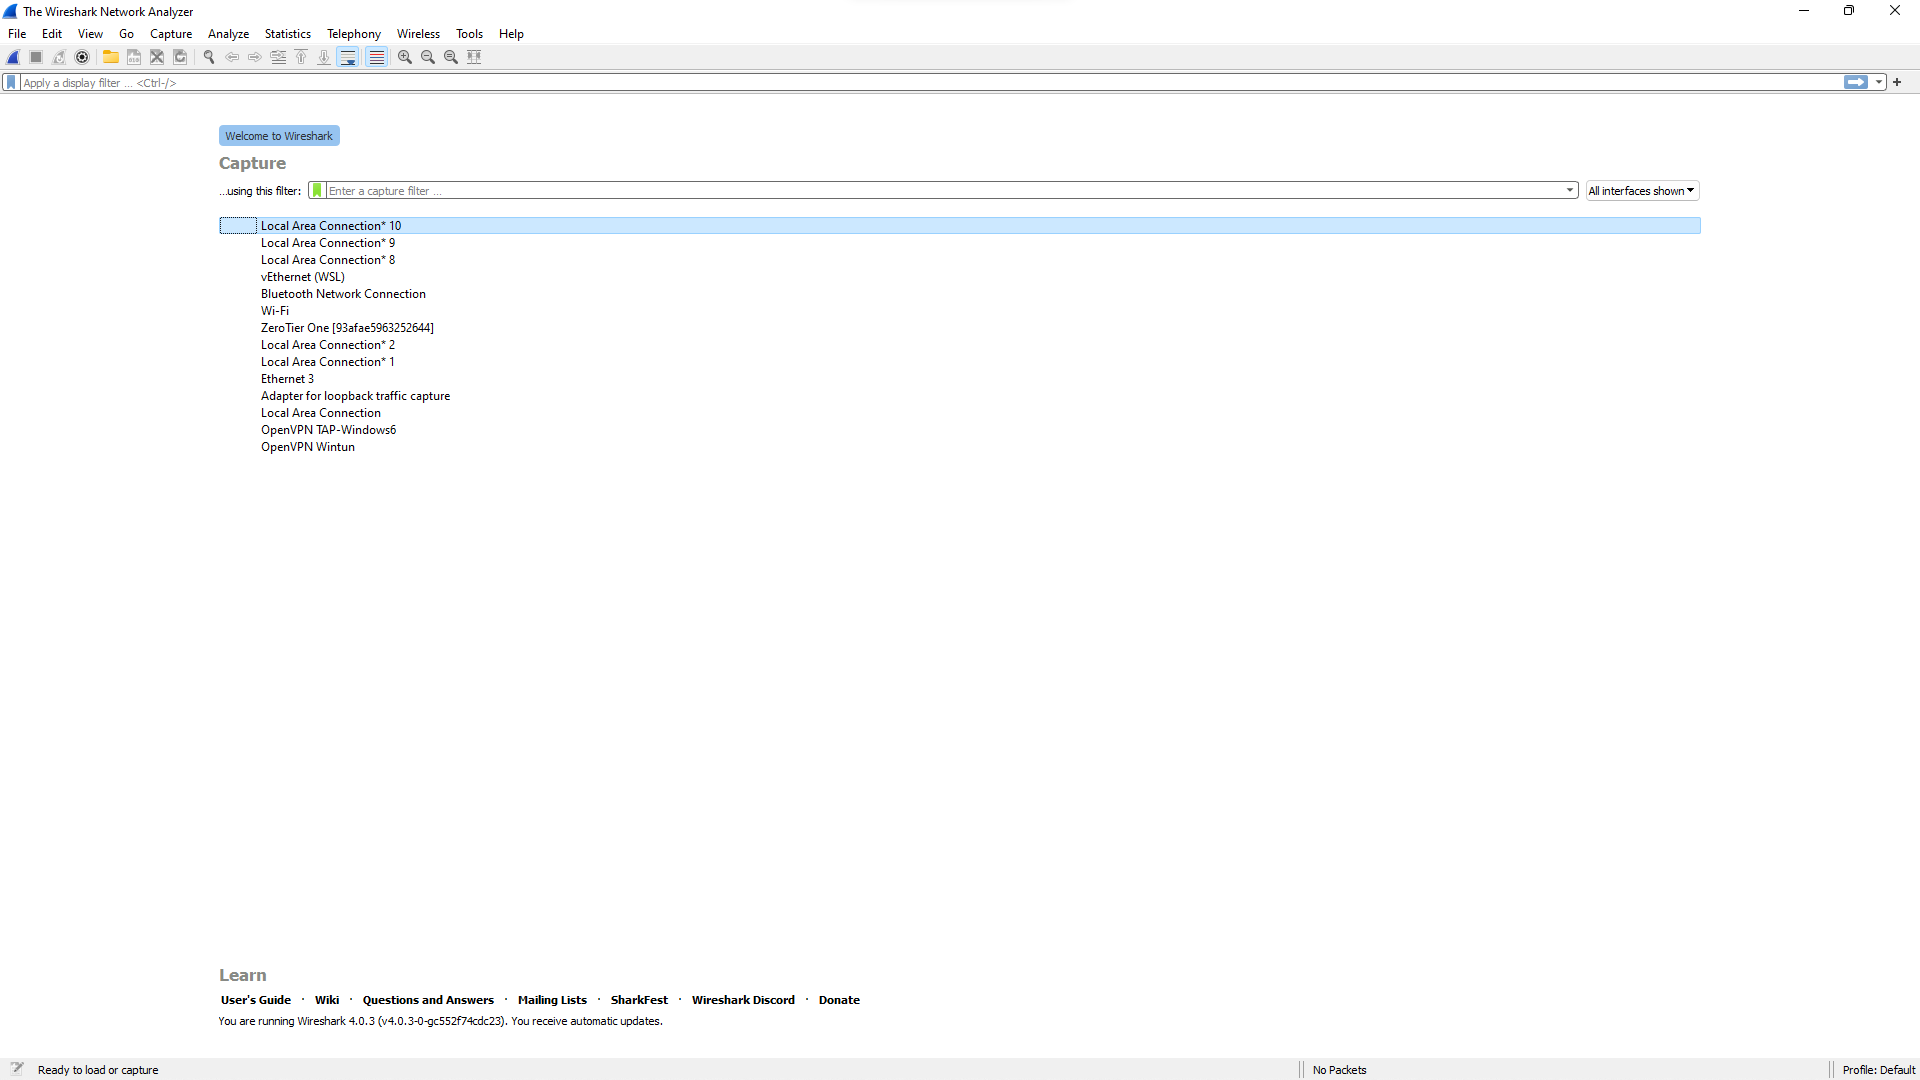
\includegraphics[width=0.85\textwidth]{03_0001}
    \caption{Запускаем сниффер}
    \label{img:0001}
  \end{figure}

  \begin{figure}[H]
    \centering
    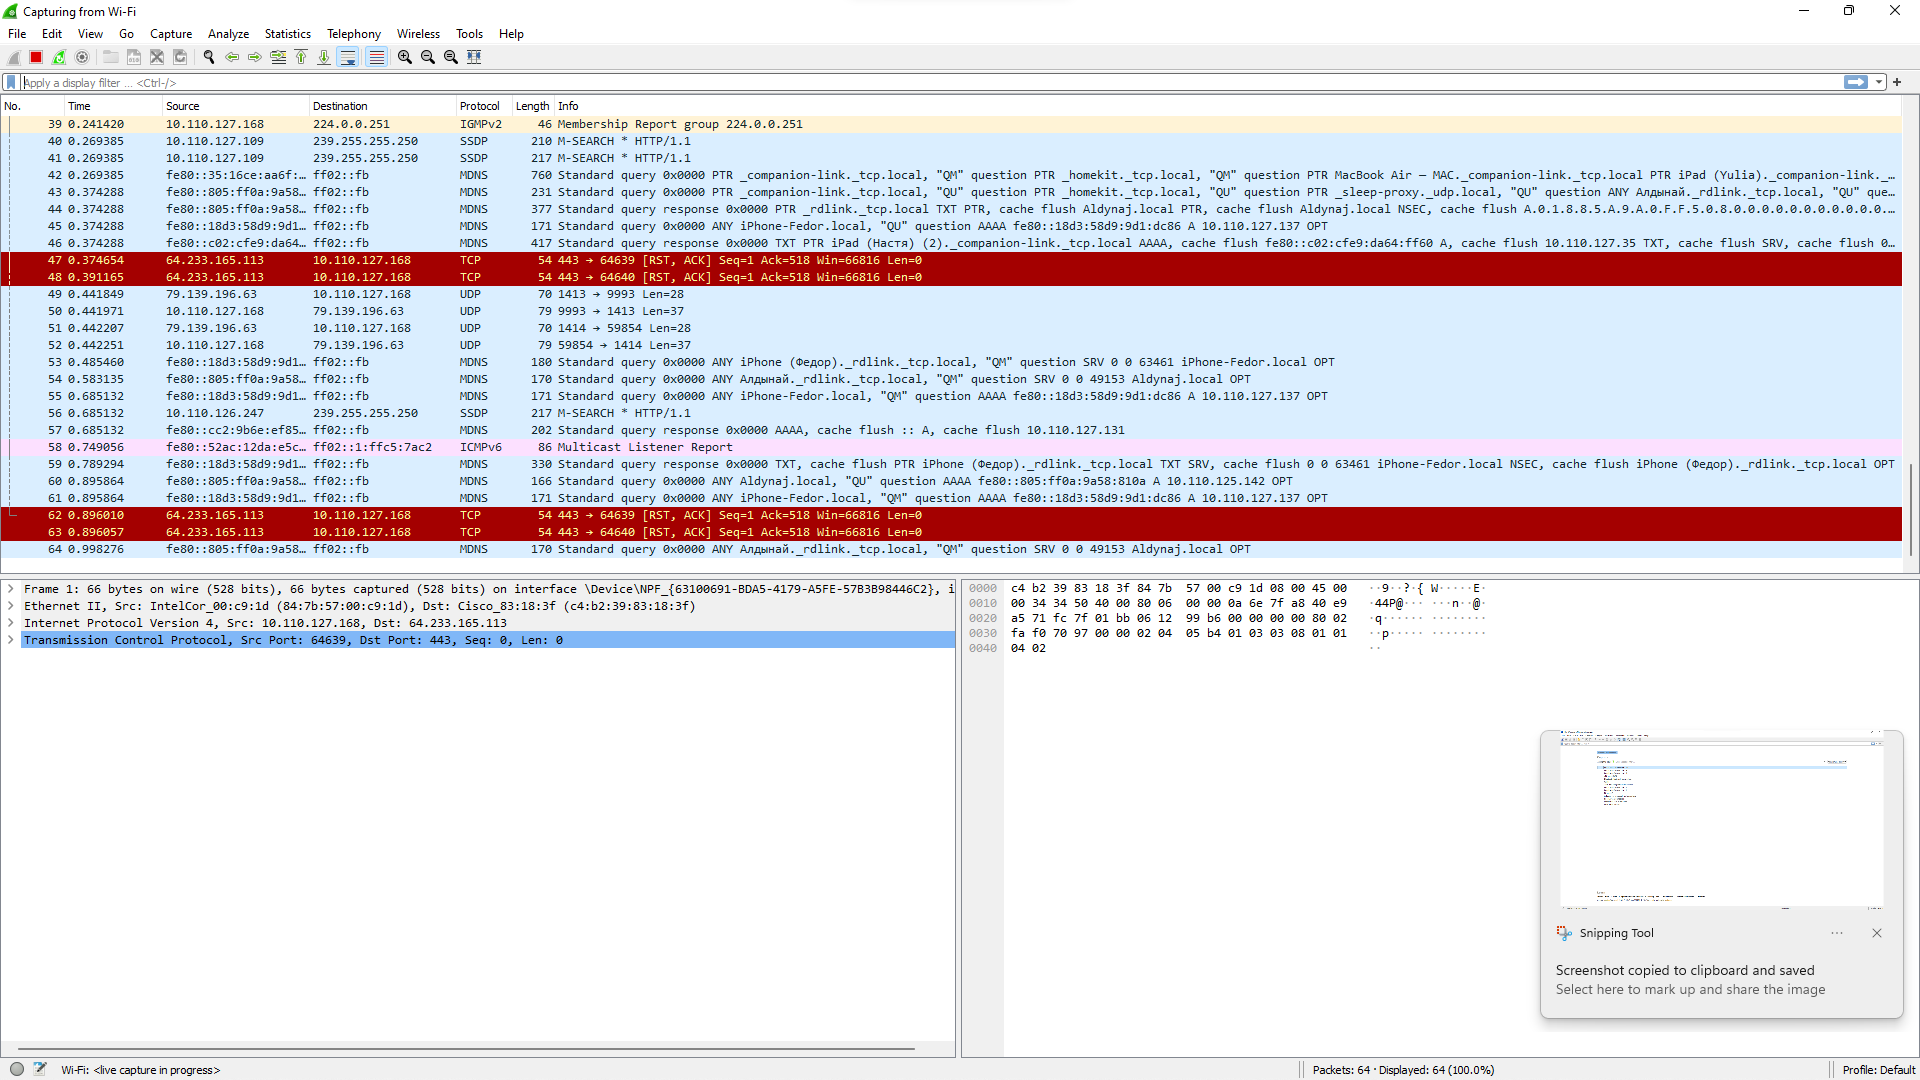
\includegraphics[width=0.85\textwidth]{03_0002}
    \caption{Начинаем захват пакетов}
    \label{img:0002}
  \end{figure}

  Для анализа потребуется пакет, переданный с помощью Ethernet II и IPv4, проще
  всего поймать такой, выполнив HTTP-запрос. Для примера, зайдем на страницу 
  с расписанием занятий:
  
  \begin{figure}[H]
    \centering 
    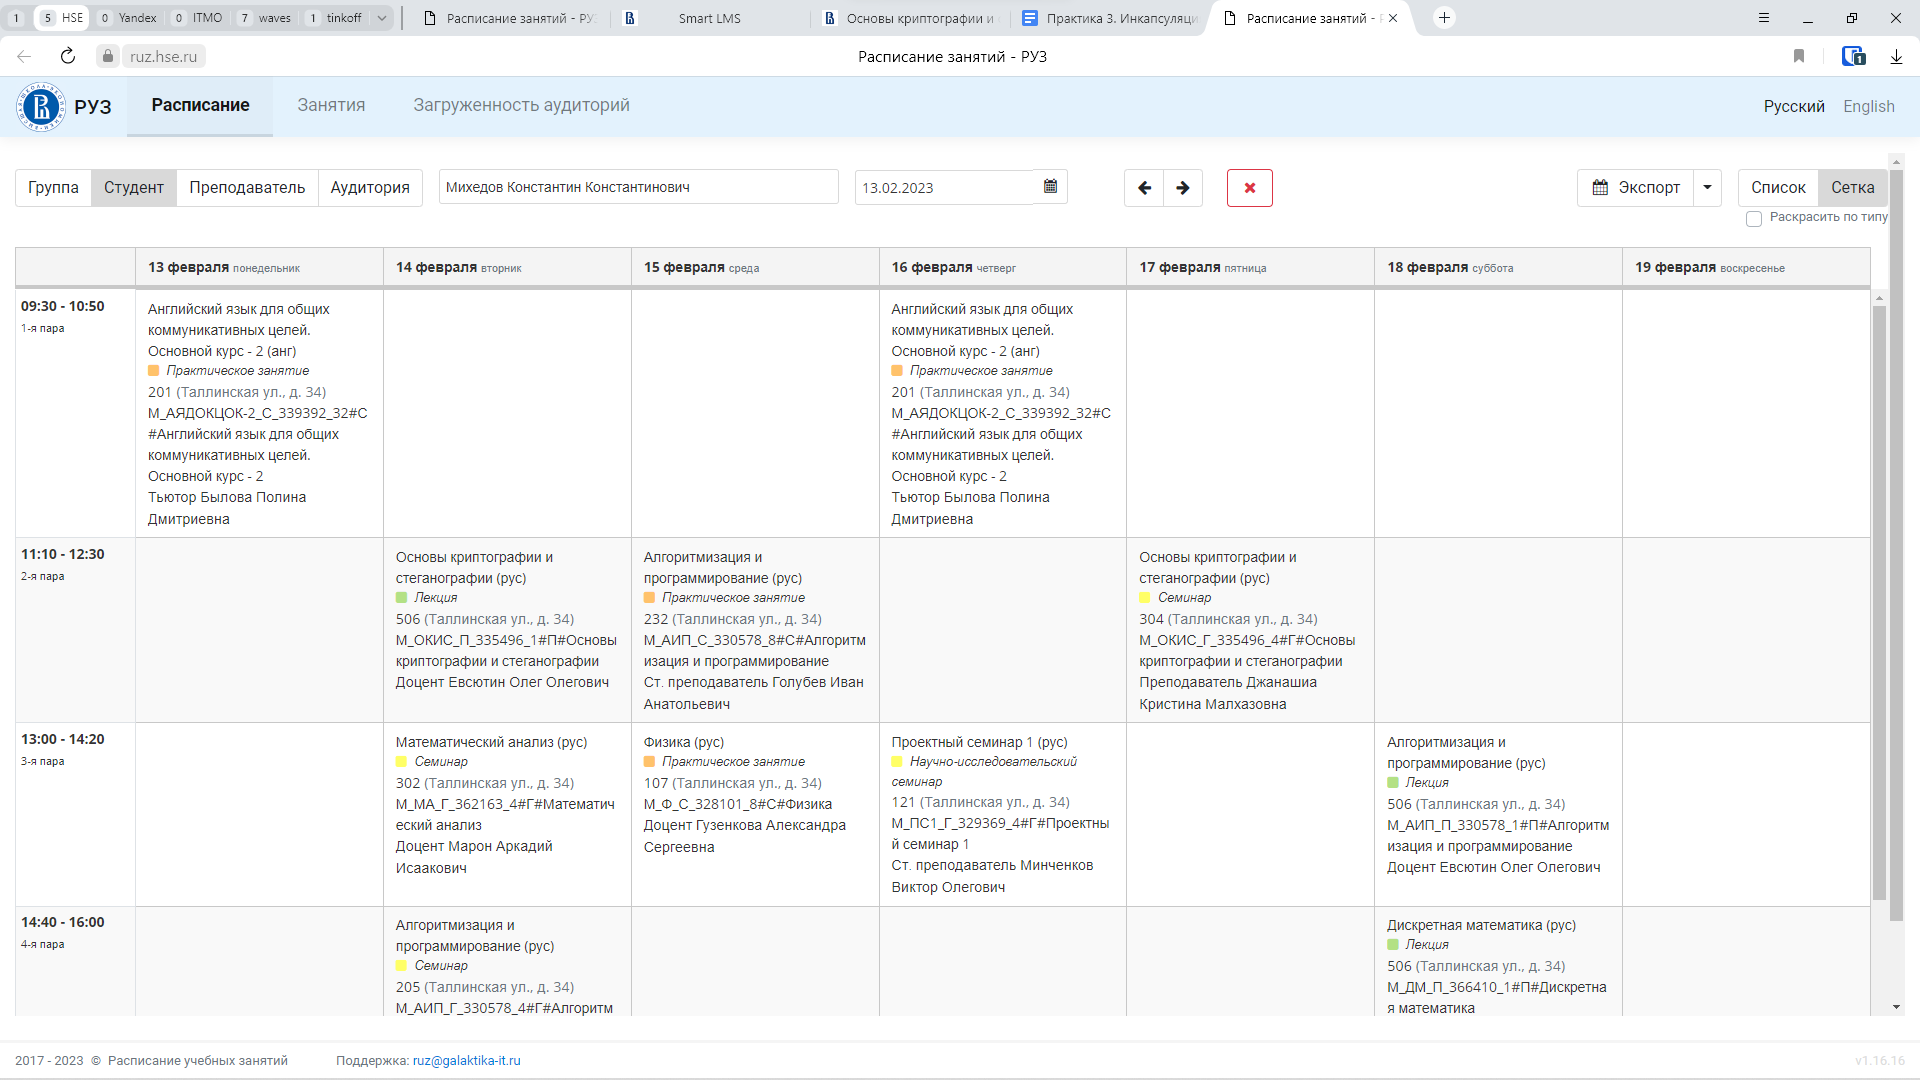
\includegraphics[width=0.85\textwidth]{03_0003}
    \caption{Используем браузер для выполнения HTTP-запросов}
    \label{img:0003}
  \end{figure}

  \begin{figure}[H]
    \centering
    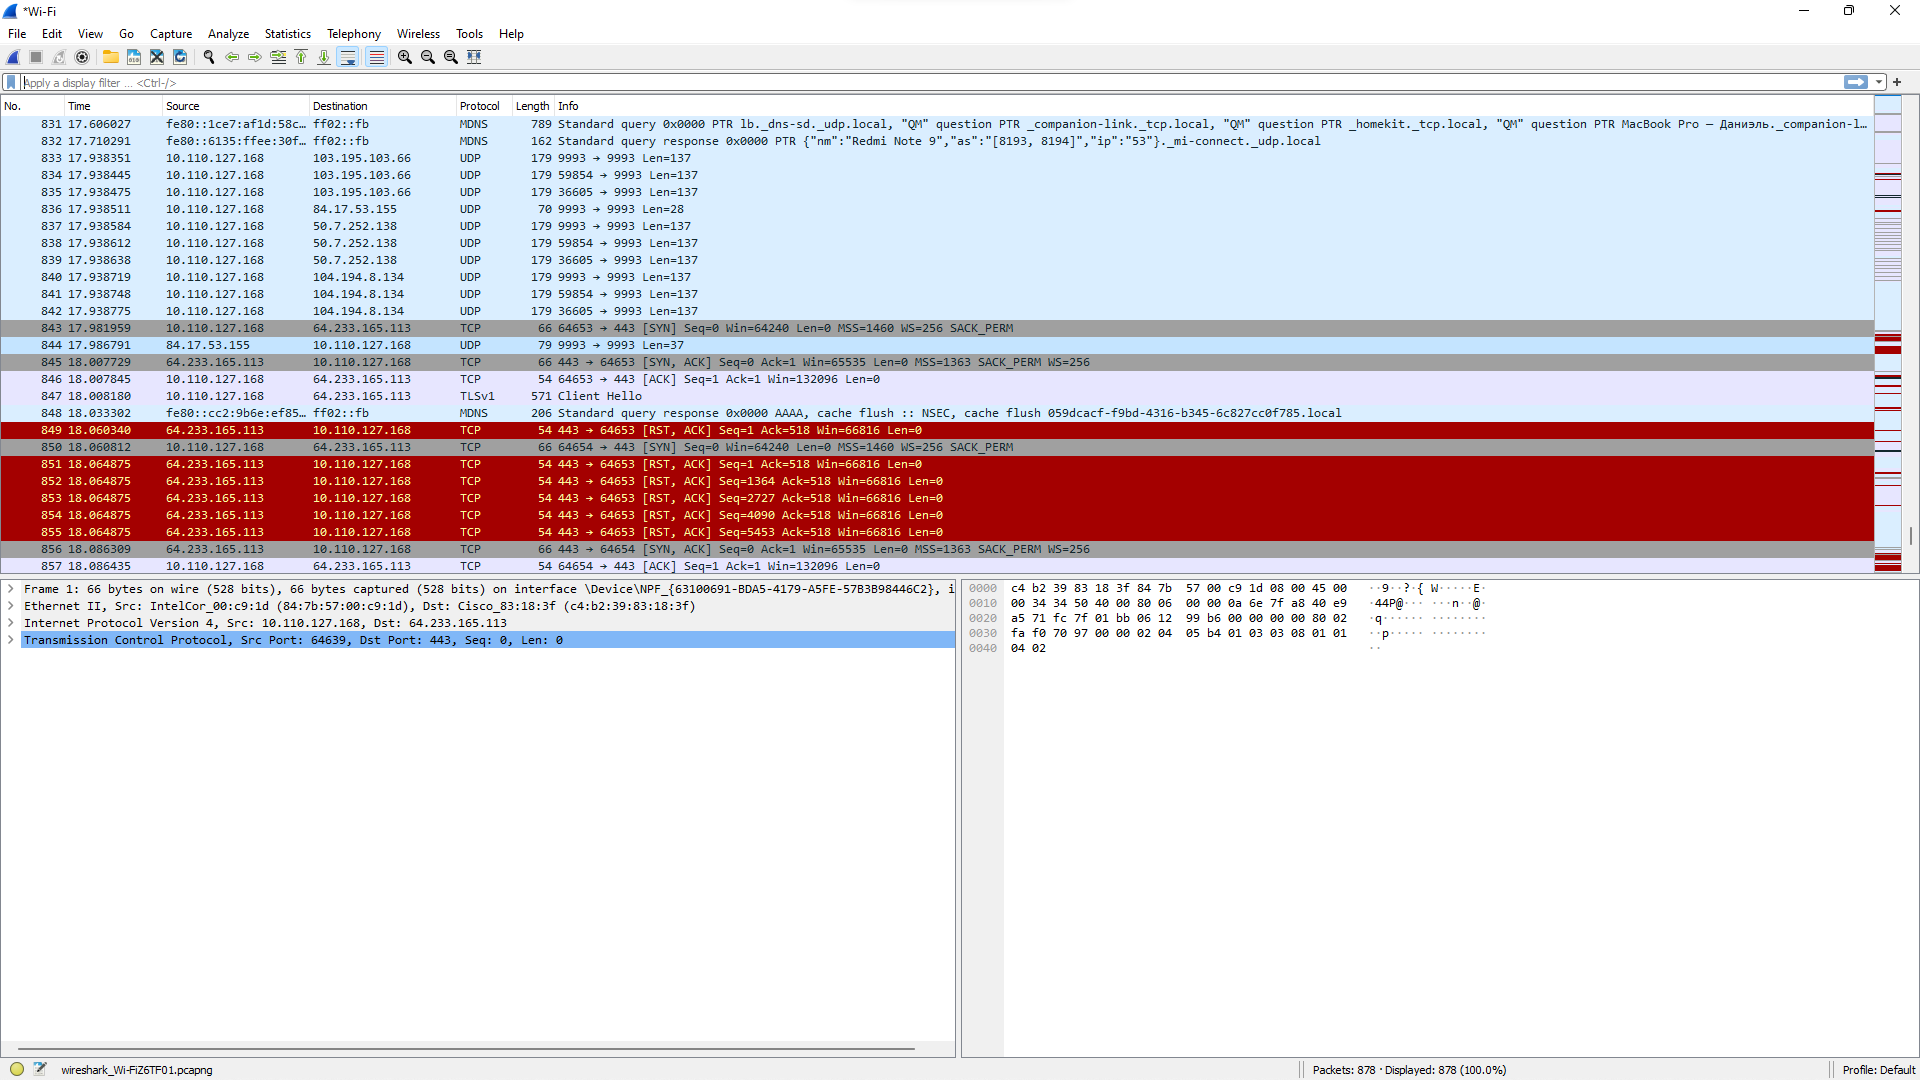
\includegraphics[width=0.85\textwidth]{03_0004}
    \caption{Останавливаем захват пакетов}
    \label{img:0004}
  \end{figure}

  Чтобы быстрее найти подходящий пакет, можно воспользоваться следующим фильтром: \textit{ip.version == 4}
  \begin{figure}[H]
    \centering
    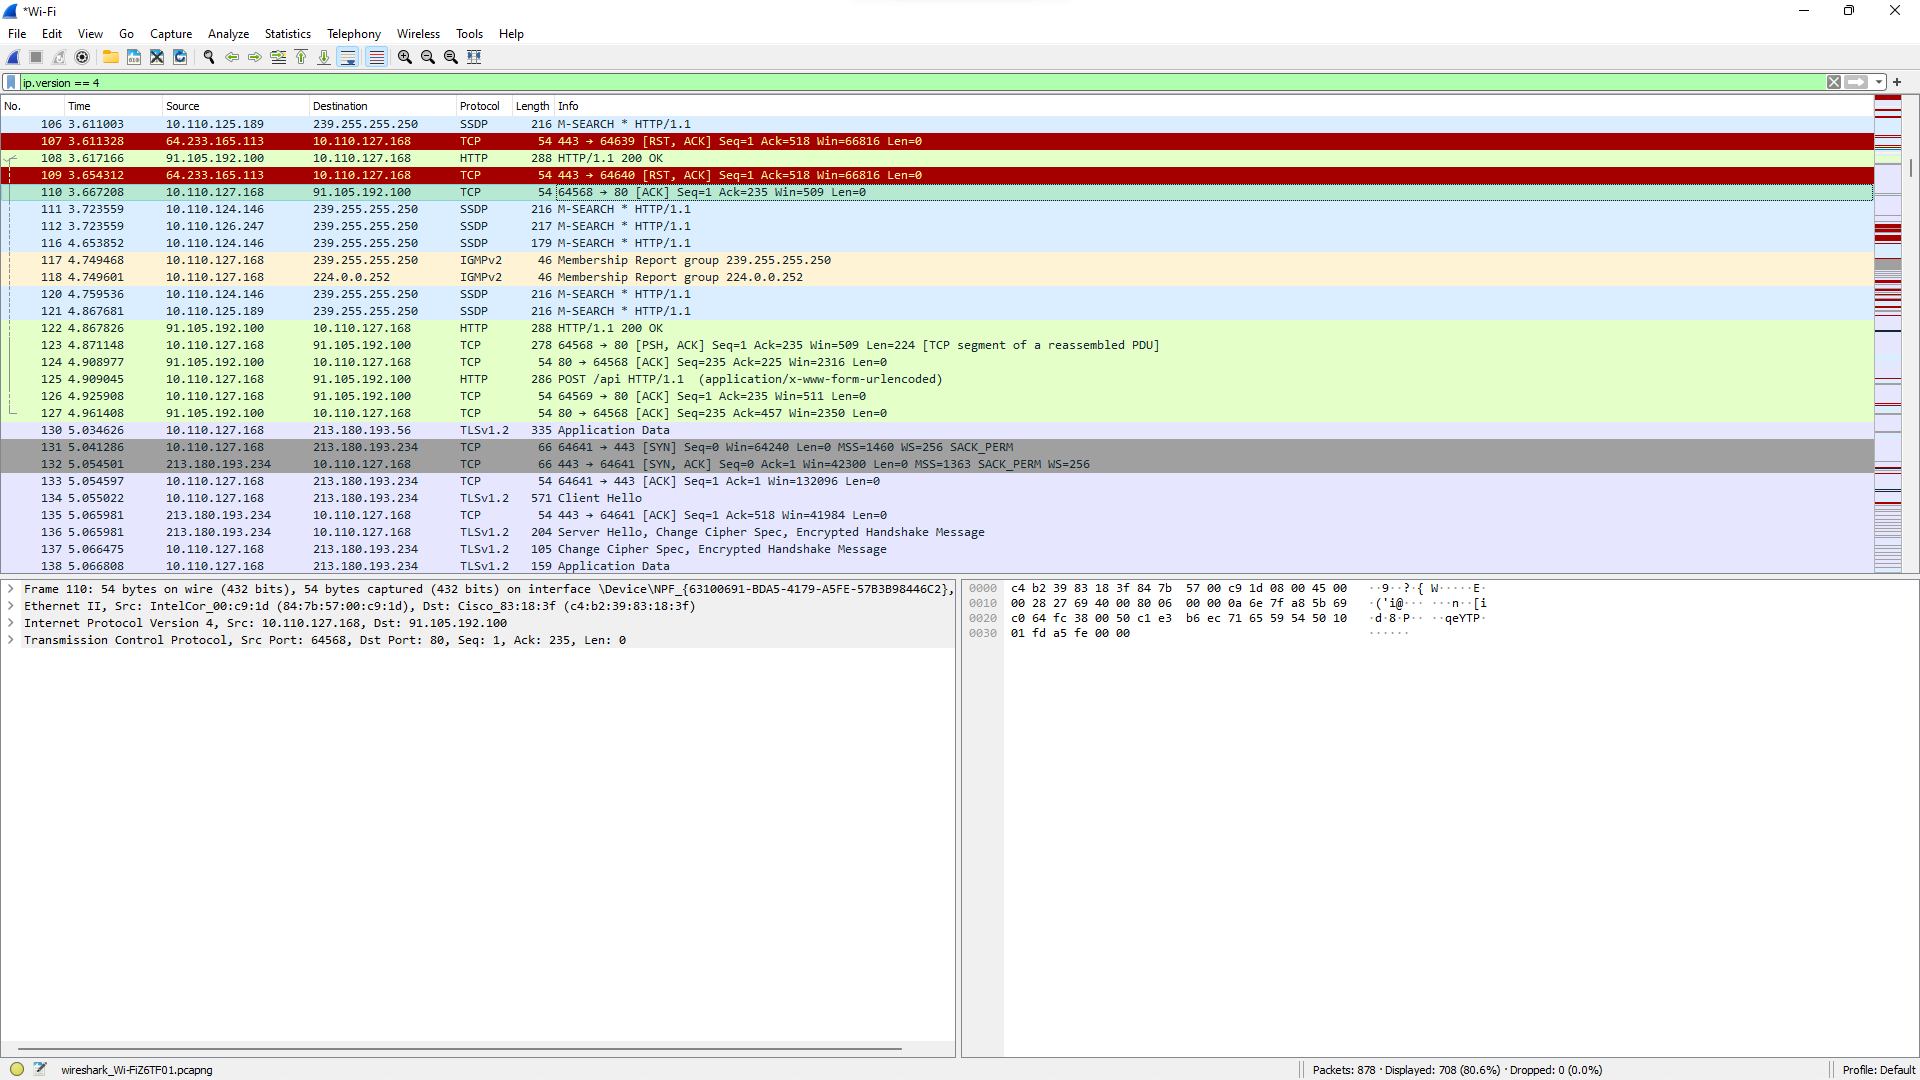
\includegraphics[width=0.85\textwidth]{03_0005}
    \caption{Подходящий пакет найден}
    \label{img:0005}
  \end{figure}

  \subsection{Анализ Ethernet II заголовка}

  Откроем окно с информацией о выбранном пакете и скопируем оттуда информацию 
  об Ethernet заголовке данного пакета:

  \begin{figure}[H]
    \centering 
    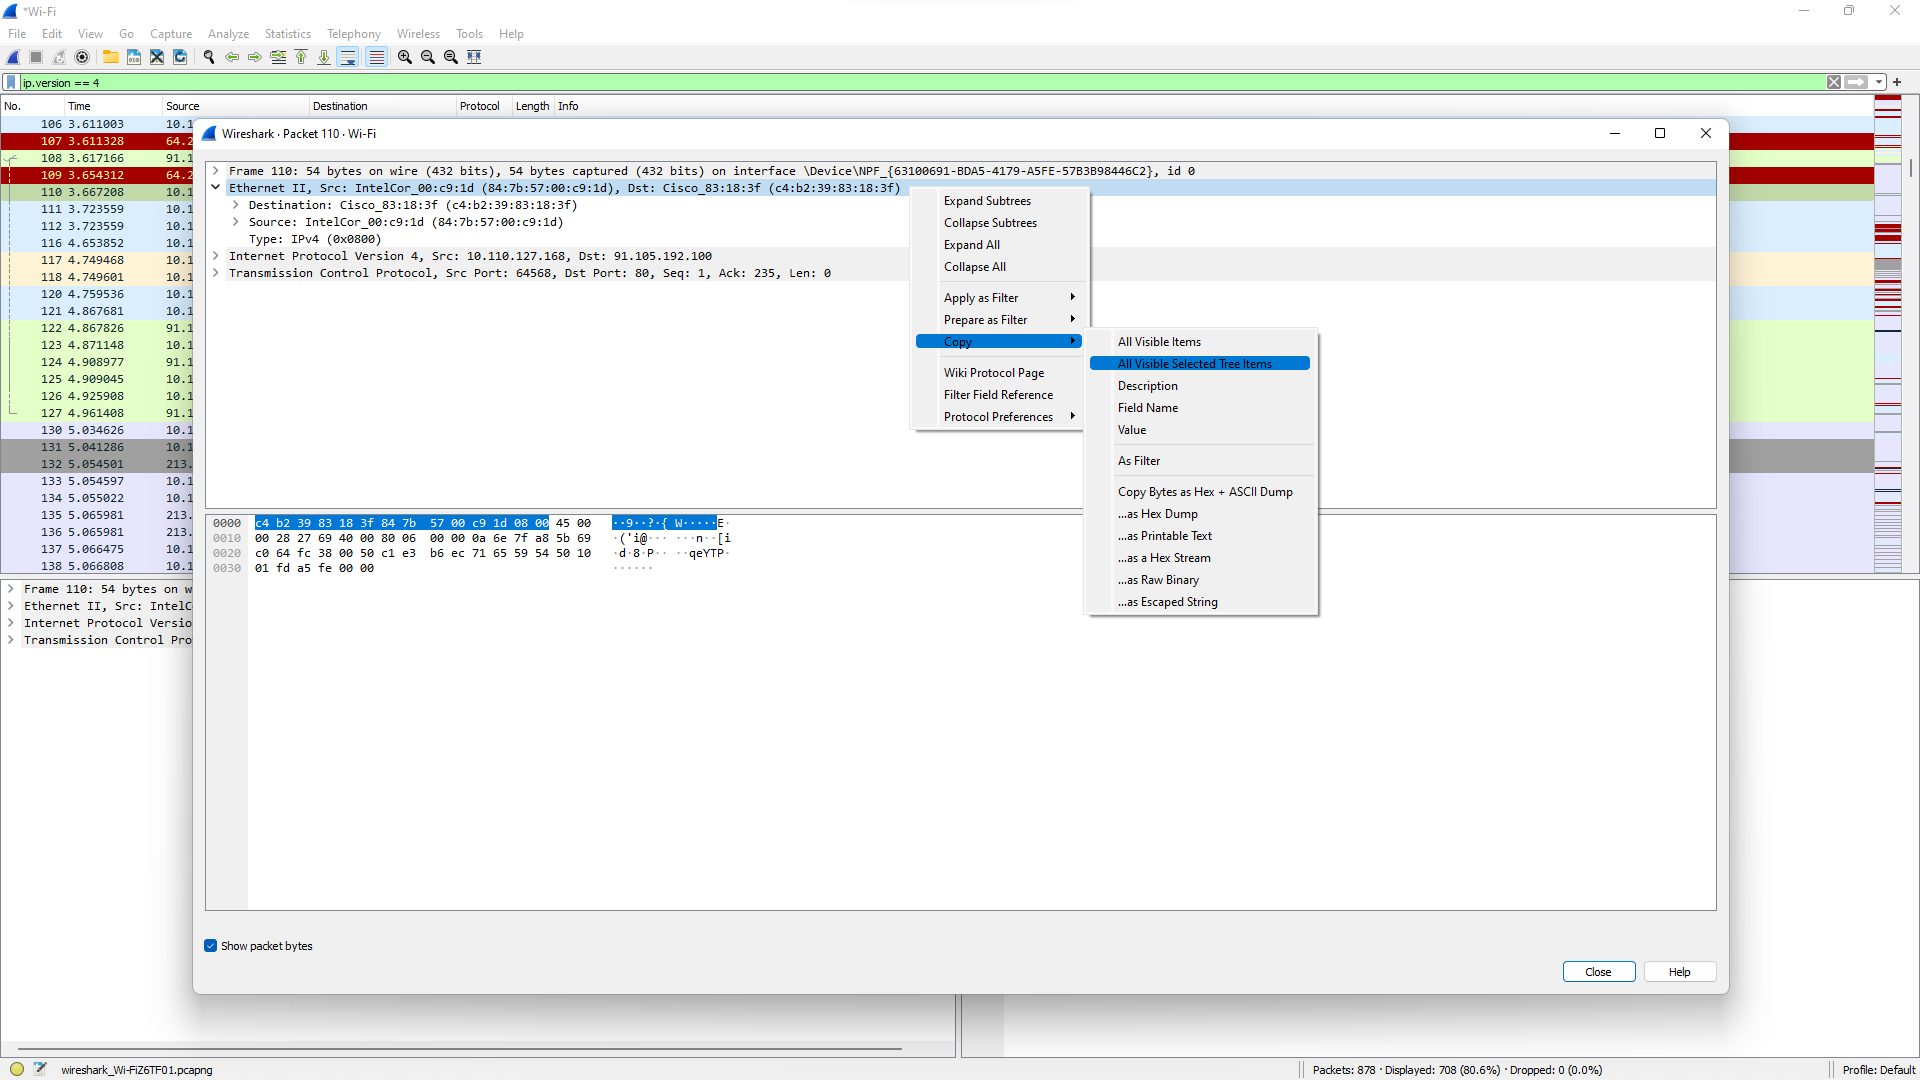
\includegraphics[width=0.85\textwidth]{03_0006}
    \caption{Копируем информацию о Ethernet заголовке}
    \label{img:0006}
  \end{figure}

  Полученная информация выглядит следующим образом:

  \begin{listing}[H]
    \begin{minted}{text}
      Ethernet II, 
          Src: IntelCor_00:c9:1d (84:7b:57:00:c9:1d),
          Dst: Cisco_83:18:3f (c4:b2:39:83:18:3f)
      Destination: Cisco_83:18:3f (c4:b2:39:83:18:3f)
      Source: IntelCor_00:c9:1d (84:7b:57:00:c9:1d)
      Type: IPv4 (0x0800)
    \end{minted}  
  \end{listing}

  Поподробнее рассмотрим информаию о данном заголовке:
  \begin{enumerate}
    \item {
      \textbf{Ethernet II} - данная часть указывает на стандарт Ethernet кадра,
      точнее - на его вторую версию (повсеместно используемую в сетевом оборудовании).
    }
    \item {
      \textbf{Destination} или \textbf{Dst} - MAC-адрес устройства-получателя

      В данном случае видно, что пакеты уходят к устройству, имеющему
      адрес c4:b2:39:83:18:3f.
      Причем \textit{Wireshark} самостоятельно определил производителя сетевого 
      устройства получателя - \textit{Cisco}
    }
    \item {
      \textbf{Source} или \textbf{Src} - MAC-адрес устройства-отправителя

      По заголовку понятно, что отправитель имел адрес 84:7b:57:00:c9:1d.
      По этому же адресу определяется vendor - \textit{IntelCor}.
    }
    \item {
      \textbf{Type} - указывает на протокол верхнего уровня, данные которого 
      находятся в текущем кадре. Установленное значение 0x0800 зарезервированно
      для протокола IPv4 (это также подсвечено \textit{Wireshark}).
    }
    \item {
      Поле данных здесь не отображается, но позже также будет частично рассмотренно.
    }
    \item {
      \textbf{FCS} - контрольная сумма данных фрейма также не отображается.
    }
  \end{enumerate}

  \subsection{Анализ IPv4 заголовка}

  Из окна с информацией о необходимом пакете скопируем данные оп IP заголовке 
  этого пакета:
  
  \begin{figure}[H]
    \centering 
    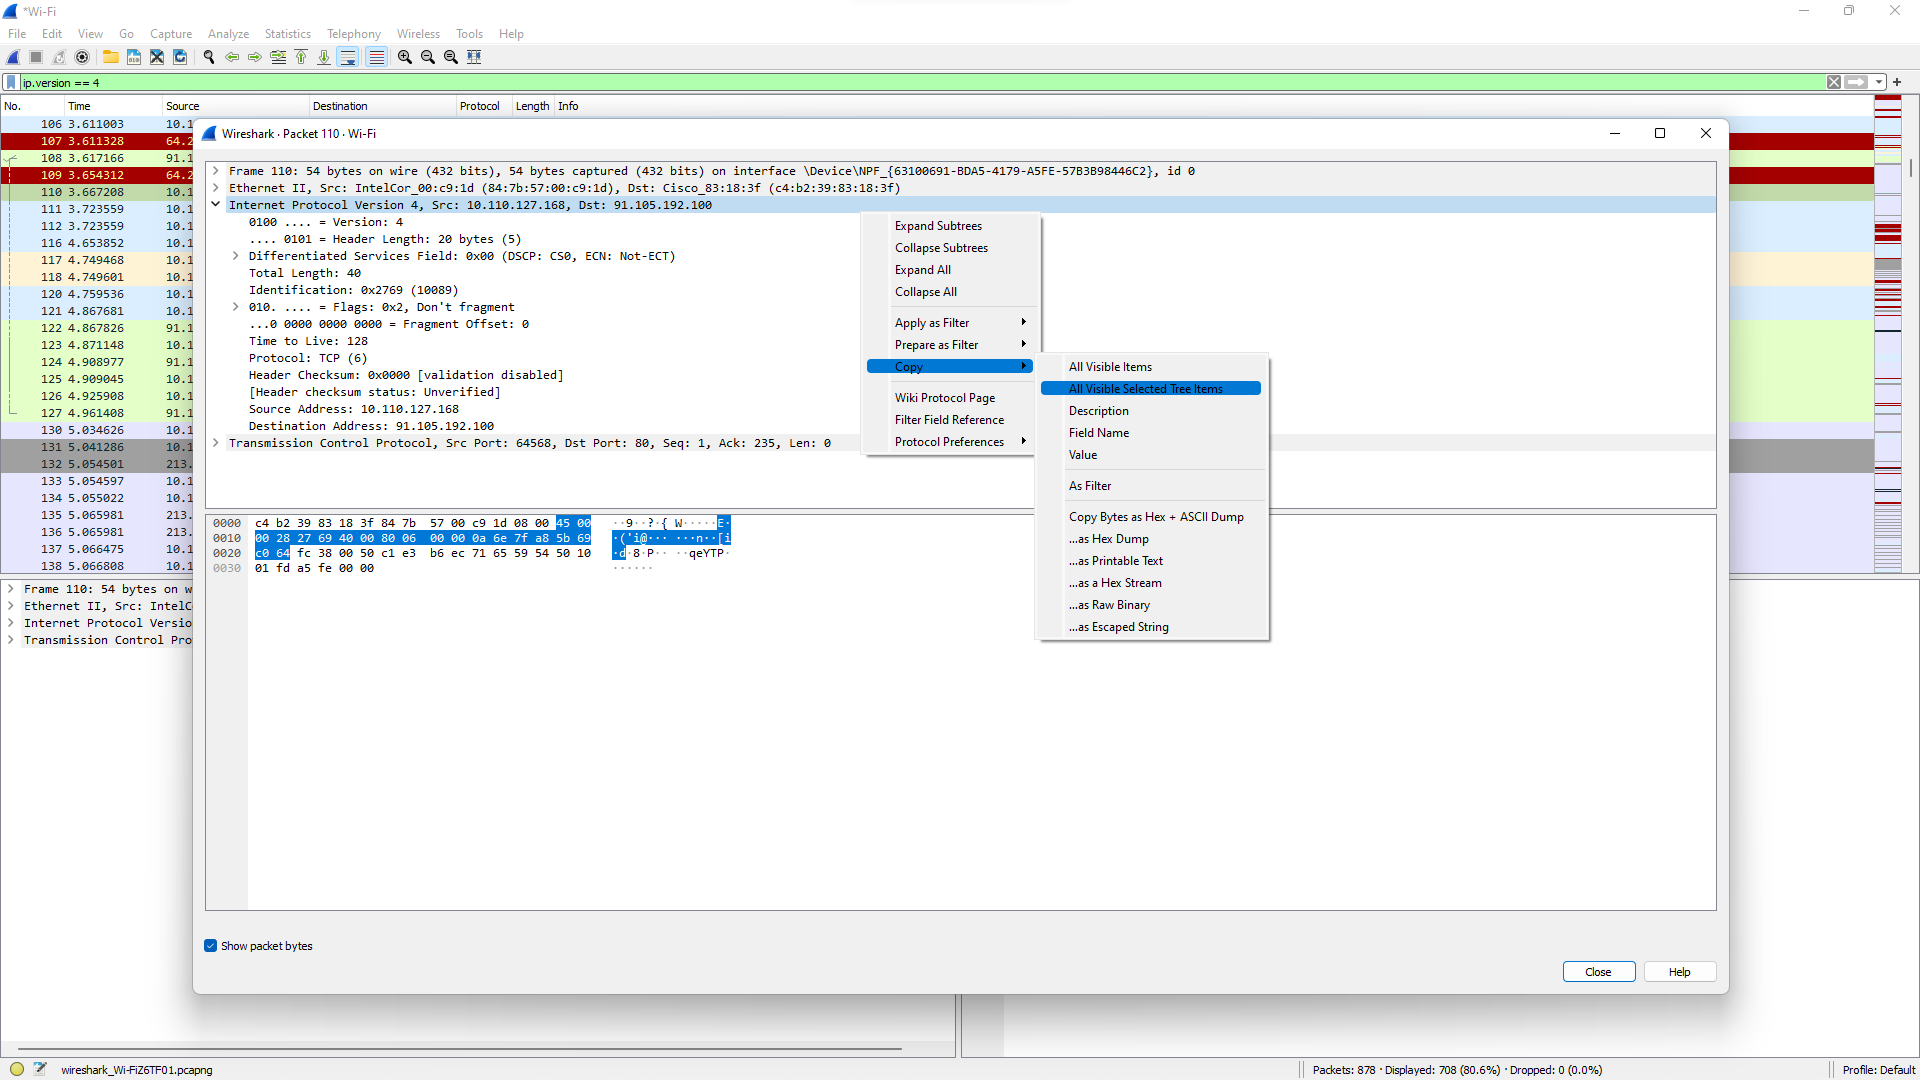
\includegraphics[width=0.85\textwidth]{03_0007}
    \caption{Копируем информацию о IP заголовке}
    \label{img:0007}
  \end{figure}

  Полученная информация выглядит следующим образом:
  \begin{listing}[H]
    \begin{minted}{text}
      Internet Protocol Version 4,
        Src: 10.110.127.168,
        Dst: 91.105.192.100
      0100 .... = Version: 4
      .... 0101 = Header Length: 20 bytes (5)
      Differentiated Services Field:
        0x00 (DSCP: CS0, ECN: Not-ECT)
      Total Length: 40
      Identification: 0x2769 (10089)
      010. .... = Flags: 0x2, Don't fragment
      ...0 0000 0000 0000 = Fragment Offset: 0
      Time to Live: 128
      Protocol: TCP (6)
      Header Checksum: 0x0000 [validation disabled]
      [Header checksum status: Unverified]
      Source Address: 10.110.127.168
      Destination Address: 91.105.192.100
    \end{minted}
  \end{listing}

  Подробнее рассмотрим этот заголовок:
  \begin{enumerate}
    \item {
      Первый байт заголовка - 01000101

      Первые 4 бита данного байта указывают на версию протокола IP:
      в нашем случае $0100_2 = 4$, следовательно используется IPv4.

      Оставшиеся 4 байта показывают, сколько 32-битных слов содержится в 
      заголовке. Для текущего заголовка $0101_2 = 5$, следовательно сам 
      заголовок состоит из 5 32-битных слов, то есть из 20 байт.
    }
    \item {
      Байт дифференцируемого обслуживания

      Следующие 8 бит выделены для него и соответсвенно равны 
      00000000.
      
      Первые 3 бита из этого набора характеризуют
      приоритет пакета, в данном случае $000_2 = 0$, то есть 
      приоритет текущего пакета самый низкий из всех возможных.
    
      Следующие три бита определяют критерии выбора маршрута,
      в частности первый бит отвечает за минимизацию задержку (D),
      второй - за максимизацию пропускной способности (T), а третий -
      за надежность доставки (R). Все эти биты имееют нулевое значение,
      поэтому какие-то особые правила маршрутизации к данному пакету 
      применяться не будут.

      Оставшиеся два байта отвечают за за уведомления о перегруженности.
      Оба байта установлены в 0, следовательно данным пакетом такие уведомления 
      просто не поддерживаются.
    }
    \item {
      \textbf{Total length} - общая длина пакета (с учетом заголовка).
      Данное поле содержит в себе значение 40 (измеряется в байтах), а так как длина заголовка по 
      ранее вычисленным значениям 20 байт, то информации в текущем пакете всего на 20 байт.
    }
    \item {
      \textbf{Identification} - идентификатор пакета, инкрементируется при каждой
      отправке, поэтому по значению данного поля можно сделать вывод, что изучаемый
      пакет был отправлен 10089-ым.
    }
    \item {
      \textbf{Flags} - флаги для идентификации фрагмента

      Для данного поля зарезервированно 3 бита, хотя по факту используются
      лишь второй и третий. Если 1 стоит во втором бите (как и в текущем пакете),
      то текущий пакет не может быть фрагментирован и несет в себе всю 
      информацию сразу, если же в 1 установлен 
      третий бит - данный пакет разбит на фрагменты.
    }
    \item {
      \textbf{Fragment Offset} - поле смещения фрагмента
      
      Необходимо выстроения полученных фрагментов в правильном порядке.
      Так как для данного пакета фрагментирование не используется,
      данное поле установлено в 0.
    }
    \item {
      \textbf{Time To Live} - время жизни пакета 

      Характеризует время, в течении которого пакет может передаваться по сети.
      Для текущего пакета значение TTL - 128 (измеряется в количестве переходов
      между участками маршрутизации).
    }
    \item {
      \textbf{Protocol} - идентификатор протокола верхнего уровня

      По данному полю видно, что вышележищий уровень использует протокол TCP.
    }
    \item {
      \textbf{Header Checksum} - контрольная сумма заголовка текущего пакета 

      Используется для проверки целостности заголовка. В данном случае 
      значение данной суммы равно нулю, что соответсвует отключенной
      проверке целостности заголовка.
    }
    \item {
      \textbf{Source Address} - IP адрес отправителя пакета. По данному полю видно,
      что пакет был отправлен с устройства, IPv4 которого 10.110.127.168
    }
    \item {
      \textbf{Destination Address} - IP адрес получателя пакеты. Видно, что 
      изучаемый пакет был отправлен по адресу 91.105.192.100
    }
  \end{enumerate}

  \newpage
  \section{Вывод}

  В ходе данной лабораторной работы мне удалось лучше разобраться в инкапсуляции
  пересылаемых данных, а также узнать, какие данные дополнительно накладывают 
  протоколы IP и Ethernet, научиться их читать.

\end{document}
